%=============================================================================
% ..... THIS IS chapter{TRUNCATE: ITU-T bitstream truncation tool } .....
%     Apr.2005
% ... Authors :
%        Cyril Guillaum� & St�phane Ragot - stephane.ragot@francetelecom.com
%     Revised Oct 2009: yusuke hiwasaki
%
%=============================================================================
\chapter{ITU-T Bitstream truncation tool}
%=============================================================================

%----------------------------------------------------------------------
\section{Introduction}
%----------------------------------------------------------------------

A scalable codec is a highly flexible coding technique that is
characterized by a multi-layer bitstream:
\begin{itemize}
\item The core layer provides the minimum quality. This layer is a
  minimum requirement for a decoder to operate, or otherwise the frame
  is considered lost.
\item Upper layers improves quality by increasing bitrate.
\end{itemize}

The main feature of a scalable codec lies in bit rate flexibility.
The bitrate can be adjusted between minimal and maximal values by any
component in the communication chain. For instance, to cope with
network congestion, the bitrate can be adjusted on a frame by frame
basis.

The bitrate modification is very simple as it consists of cutting the
bitstream at the right rate, i.e., stripping bits. Apart from this
straightforward truncation, no signal processing is required.

To simulate this functionality, a bitstream truncation tool (truncate)
was introduced into STL2005. G.192 bitstreams (with or without sync
header), G.192 byte-oriented bitstreams (with or without sync header)
and binary (compact) bitstreams can be processed with this tool.

%----------------------------------------------------------------------
\section{Description of the algorithm}
%----------------------------------------------------------------------

This tool truncates the bitstream at the desired bitrate (see
Figure~\ref{trunc-principle}). For each frame of an input bitstream,
this tool performs the following operations :
\begin{enumerate}
\item Read the synchronization word and copy it to the output bitstream;
\item Write the new frame length word equal to the number N2 of 
      bits to copy to the output bitstream (N2 depends on the 
      desired bit rate);
\item Read the N1 words of the input bitstream and copy the first 
      N2 16-bit words representing the first N2 bits of the input to
      the output bitstream. 
\end{enumerate}

%------------------------------------------------------------------------
\begin{figure}[h]
  \begin{center}
    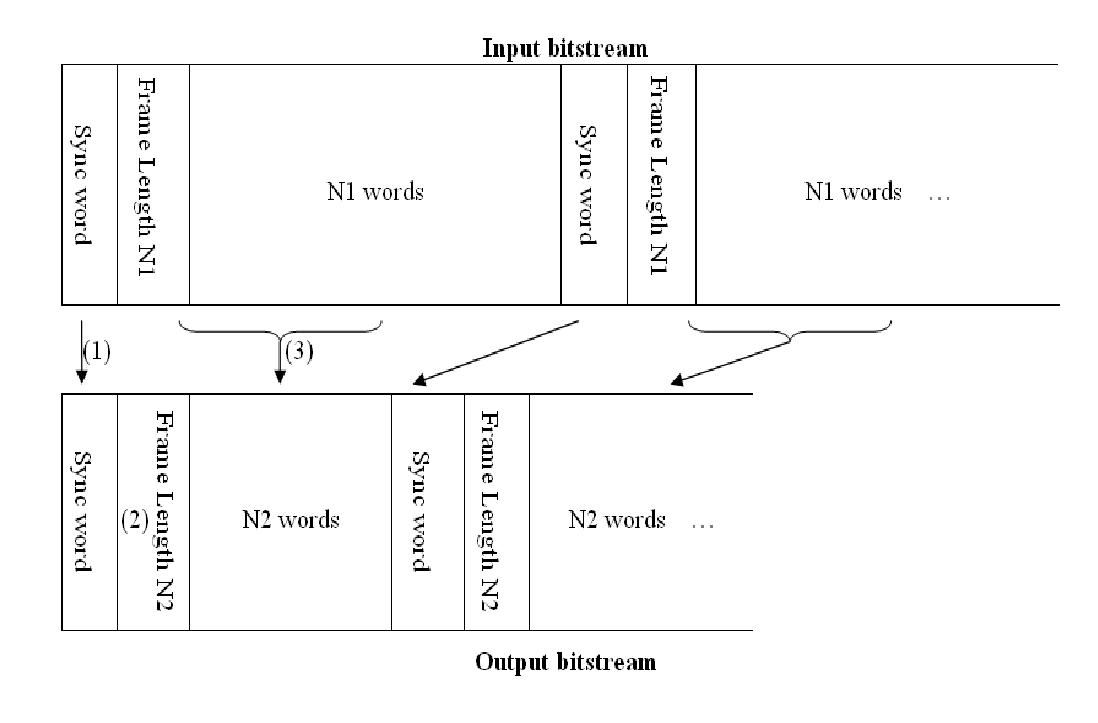
\includegraphics[width=16cm]{trunc-desc}
    \caption{Bitstream truncation principle.\label{trunc-principle}}
  \end{center}
\end{figure}
%------------------ End of figure ----------------------------------

For example, one frame of the input bitstream will comprise 640 bits
for a 32 kbit/s codec operating a frame size of 20 ms. To truncate
the 32 kbit/s input bitstream to 14 kbit/s, the output bitstream
frame length will be set to 280 for each frame. Only the first 280
words of the 640 words of the input bitstream will be copied in the
output bitstream while the last 360 words will be discarded.

%----------------------------------------------------------------------
\section{Implementation}
%----------------------------------------------------------------------

%-.-.-.-.-.-.-.-.-.-.-.-.-.-.-.-.-.-.-.-.-.-.-.-.-.-.-.-.-.-.-.-.-.-.-.
\subsection{\tt trunc}

{\bf Syntax: }

{\tt
\#include "trunc-lib.h"\\
void trunc \ttpbox{130mm}{(short {\em syncWord}, short {\em
outFrameLgth}, short* {\em inpFrame}, short* {\em outFrame}); }}

{\bf Prototype: }    trunc-lib.h

{\bf Description: }

This routine copies the {\em syncWord} and the first {\em
outFrameLgth} words of the input frame {\em inpFrame} to the
output frame {\em outFrame}.

{\bf Variables: }
\begin{Descr}{\DescrLen}
\item[\pbox{20mm}{\em syncWord}] %%\rulex{1mm}\\
        synchronization word to write to the output frame;

\item[\pbox{20mm}{\em outFrameLgth}] %%\rulex{1mm}\\
        length of the output frame;

\item[\pbox{20mm}{\em inpFrame}] %%\rulex{1mm}\\
        input frame to truncate;

\item[\pbox{20mm}{\em outFrame}] %%\rulex{1mm}\\
        output frame;
\end{Descr}

%-.-.-.-.-.-.-.-.-.-.-.-.-.-.-.-.-.-.-.-.-.-.-.-.-.-.-.-.-.-.-.-.-.-.-.
\subsection{Tests and portability}

Compiled and tested on a PC (Windows) platform with MS Visual C++
6.0. A bitrate file can be obtains with the tool gen\_rate contain in
EID module.


%----------------------------------------------------------------------
\section{Example code}
%----------------------------------------------------------------------

A demonstration program {\em truncate.c} illustrates the use of this
module to truncate a bitstream to the desired bitrate.
